\documentclass[10pt,twocolumn]{article}

\usepackage[T1]{fontenc}
\usepackage[utf8]{inputenc}
\usepackage{mathptmx}
\usepackage{microtype}
\usepackage[a4paper,top=1.45cm,bottom=1.55cm,left=1.45cm,right=1.45cm,columnsep=0.55cm]{geometry}
\usepackage{graphicx}
\usepackage{booktabs}
\usepackage{array}
\usepackage{amsmath}
\usepackage{url}
\usepackage[hidelinks]{hyperref}
\usepackage[font=small,labelfont=bf]{caption}
\usepackage{xcolor}

\setlength{\parindent}{1em}
\setlength{\parskip}{0pt}
\setlength{\textfloatsep}{7pt plus 2pt minus 2pt}
\setlength{\floatsep}{6pt plus 2pt minus 2pt}
\setlength{\intextsep}{6pt plus 2pt minus 2pt}
\captionsetup{belowskip=0pt,aboveskip=3pt}
\renewcommand{\refname}{Referências}
\renewcommand{\abstractname}{Resumo}

\title{\vspace{-1.1cm}\textbf{Classificação do Iris com uma MLP Implementada do Zero}\vspace{-0.35cm}}
\author{\small Felipe Duarte Silva -- GRR20231957 \qquad Paulo Henrique Jankosz -- GRR20220627\\
\small Departamento de Informática -- Universidade Federal do Paraná\\
\small Visão Computacional}
\date{}

\begin{document}
\maketitle
\vspace{-0.9cm}

\begin{abstract}
Este trabalho depura e estende uma implementação de perceptron multicamadas (MLP) construída apenas com NumPy para classificar as três espécies do conjunto Iris. Foram corrigidas inconsistências entre treino e inferência, atualização repetida de vieses e cálculo inadequado do erro. A versão final utiliza padronização, ReLU, softmax, entropia cruzada, regularização L2 e parada antecipada. Em dez divisões estratificadas, obteve acurácia média de $96{,}67\% \pm 4{,}16\%$ e F1 macro de $96{,}68\% \pm 4{,}12\%$. Um experimento controlado também evidencia overfitting quando a capacidade da rede é elevada e o conjunto de treino é reduzido.
\end{abstract}

\section{Introdução}

O perceptron multicamadas aproxima funções não lineares por meio de camadas totalmente conectadas e do algoritmo de retropropagação~\cite{rumelhart1986}. O conjunto Iris possui 150 amostras, quatro atributos morfológicos e três classes balanceadas~\cite{fisher1936}. Embora seja pequeno, ele permite observar separabilidade, convergência e sensibilidade à divisão dos dados.

O objetivo foi estudar a implementação fornecida, localizar falhas e construir uma versão reproduzível capaz de classificar bem as três espécies. O notebook executado, o código e os resultados estão disponíveis em \href{https://github.com/felipeduuartee/mlp-iris-do-zero}{github.com/felipeduuartee/mlp-iris-do-zero}.

\section{Depuração e metodologia}

\subsection{Falhas identificadas}

Na implementação original, a função de predição aplicava duas transformações lineares em sequência, mas omitia a ativação da camada oculta usada durante o treino. Além disso, cada viés era atualizado dentro do laço dos pesos, repetindo sua correção várias vezes por amostra. O erro oculto era calculado depois da alteração dos pesos de saída e o valor apresentado como MSE continha fatores arbitrários.

A correção substituiu os laços por operações matriciais e preservou a ordem correta: propagação, cálculo simultâneo dos gradientes e atualização. Um teste de diferenças centrais comparou gradientes analíticos e numéricos em quatro parâmetros; o maior erro relativo foi $1{,}21\times10^{-9}$.

\subsection{Modelo e protocolo}

A rede possui quatro entradas, uma camada oculta e três saídas. Para logits $\mathbf{z}$, a saída é
\begin{equation}
p_k=\frac{\exp(z_k-\max_j z_j)}{\sum_j\exp(z_j-\max_j z_j)},
\end{equation}
e a função objetivo combina entropia cruzada e penalização L2. A configuração final usa 12 neurônios ReLU, taxa de aprendizado $0{,}02$, lotes de 16 amostras, $\lambda=10^{-3}$, até 2500 épocas e paciência de 250 épocas.

Cada experimento separa os dados de forma estratificada em 60\% para treino, 20\% para validação e 20\% para teste. Média e desvio-padrão são estimados somente no treino. A validação seleciona a melhor época; o teste permanece isolado até a avaliação final.

\begin{table}[t]
\centering
\caption{Configurações na divisão ilustrativa (semente 1).}
\label{tab:config}
\small
\begin{tabular}{lccc}
\toprule
Configuração & Acur. & F1 & Épocas \\
\midrule
Original corrigida & 1,000 & 1,000 & 3000 \\
Padronizada + tanh & 1,000 & 1,000 & 813 \\
ReLU + L2 + parada & 1,000 & 1,000 & 1091 \\
\bottomrule
\end{tabular}
\end{table}

\section{Resultados e discussão}

\subsection{Convergência e erros}

Na execução ilustrativa, a parada antecipada executou 1091 épocas e restaurou os pesos da época 841. A acurácia e o F1 macro de teste foram 100\%, com 10 acertos em cada classe. O resultado perfeito dessa divisão não deve ser interpretado isoladamente: em dez sementes, a acurácia média foi $96{,}67\%$, com mínimo de $86{,}67\%$ e máximo de 100\%. O F1 macro médio foi $96{,}68\%$. Essa variação é esperada porque cada teste contém apenas 30 amostras.

O efeito do principal bug também foi medido na mesma rede treinada. Na divisão de semente 42, a inferência correta alcançou 100\%, enquanto a predição sem ativação obteve apenas $76{,}67\%$. Isso mostra que a falha não era apenas estilística: o procedimento de teste não representava a função aprendida.

\begin{figure*}[t]
\centering
\begin{minipage}{0.64\textwidth}
\centering
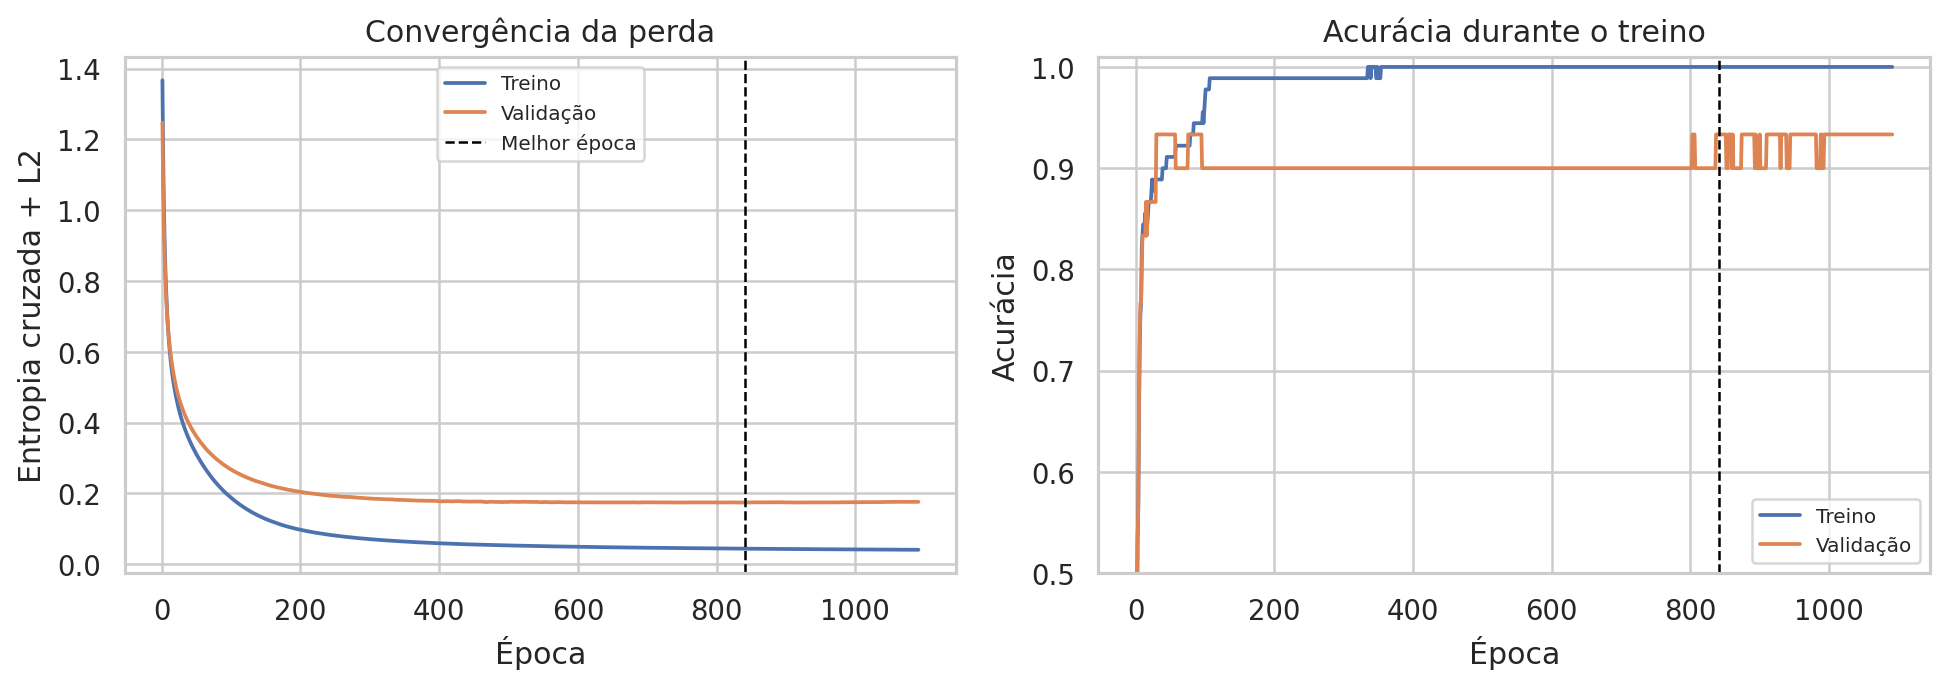
\includegraphics[width=\linewidth]{../resultados/convergencia_modelo_final.png}
\end{minipage}\hfill
\begin{minipage}{0.32\textwidth}
\centering
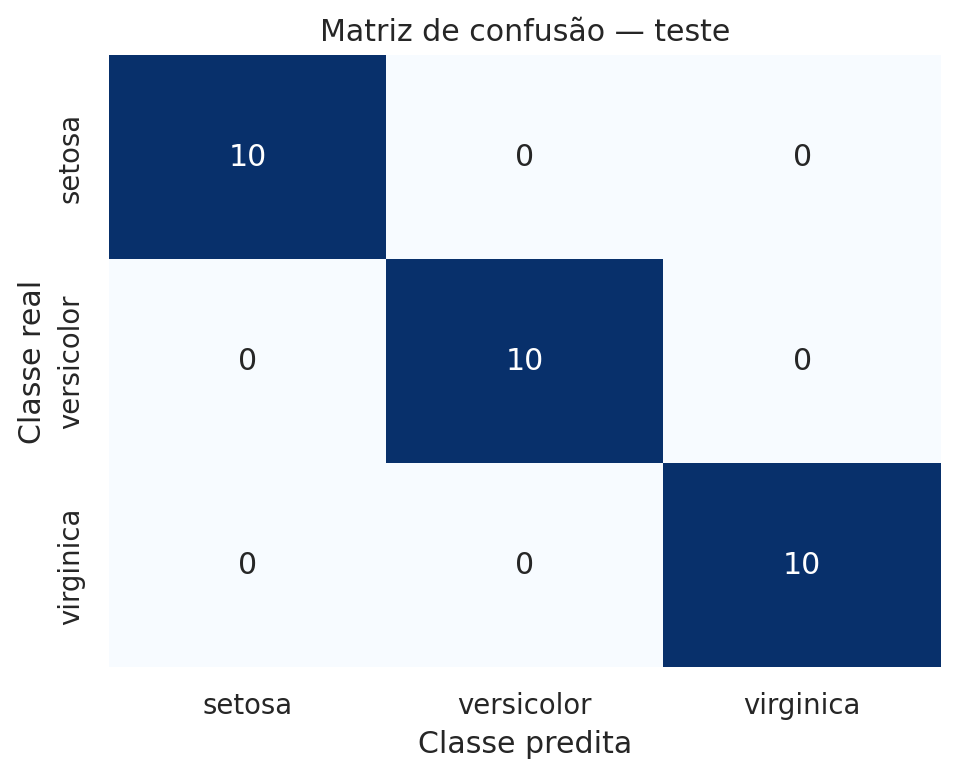
\includegraphics[width=\linewidth]{../resultados/matriz_confusao.png}
\end{minipage}
\caption{À esquerda, perda e acurácia de treino e validação do modelo final; à direita, matriz de confusão no teste da divisão ilustrativa.}
\label{fig:final}
\end{figure*}

A Fig.~\ref{fig:final} indica queda consistente da perda e estabilização da acurácia. A classe \textit{setosa} é mais facilmente separada, enquanto os casos difíceis nas demais divisões concentram-se entre \textit{versicolor} e \textit{virginica}, cujas medidas de pétala e sépala apresentam maior sobreposição.

\subsection{Overfitting}

Para expor o sobreajuste, uma rede com 64 neurônios foi treinada por 5000 épocas usando apenas 30 amostras balanceadas, sem L2 e sem parada antecipada. Ela atingiu 100\% no treino e $93{,}33\%$ na validação. Mais importante, a perda final ficou em 0,0011 no treino e 0,3193 na validação, cujo mínimo ocorreu na época 394. A divergência da Fig.~\ref{fig:overfit} mostra que continuar otimizando o treino depois desse ponto piora a generalização.

\begin{figure}[t]
\centering
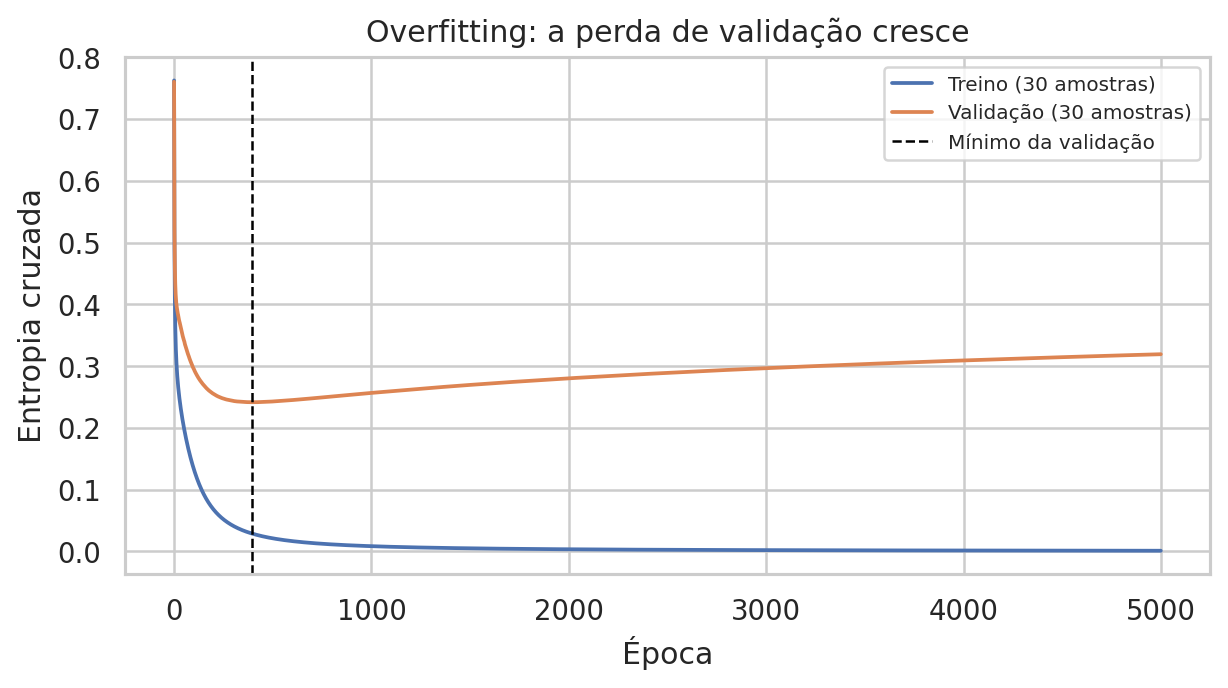
\includegraphics[width=0.98\columnwidth]{../resultados/overfitting_controlado.png}
\caption{Experimento controlado: a perda de treino continua caindo, enquanto a de validação cresce após seu mínimo.}
\label{fig:overfit}
\end{figure}

\section{Conclusão}

A implementação corrigida classifica adequadamente as três espécies e mantém todo o aprendizado da rede em NumPy. Softmax e entropia cruzada tornaram a saída multiclasse coerente; a padronização melhorou a escala dos gradientes; L2 e parada antecipada limitaram overfitting. A avaliação em dez divisões evitou concluir a partir de uma única separação favorável. Como limitação, o conjunto é pequeno e a variação entre divisões permanece relevante; por isso, médias, desvios e curvas de validação são mais informativos que um único valor de teste.

\begin{thebibliography}{9}
\small
\bibitem{fisher1936}
R. A. Fisher, ``The use of multiple measurements in taxonomic problems,'' \textit{Annals of Eugenics}, vol. 7, no. 2, pp. 179--188, 1936.

\bibitem{rumelhart1986}
D. E. Rumelhart, G. E. Hinton e R. J. Williams, ``Learning representations by back-propagating errors,'' \textit{Nature}, vol. 323, pp. 533--536, 1986.

\bibitem{goodfellow2016}
I. Goodfellow, Y. Bengio e A. Courville, \textit{Deep Learning}. MIT Press, 2016.

\bibitem{prechelt1998}
L. Prechelt, ``Early stopping -- but when?,'' em \textit{Neural Networks: Tricks of the Trade}, Springer, 1998, pp. 55--69.
\end{thebibliography}

\end{document}
